\section{Performance Evaluation}


In this section, we present the performance evaluation of our proposed approach.
We first evaluate privacy area estimation  using real world measurement data.
For detection of eavesdroppers in the front camera view, we use publicly available datasets to evaluate the accuracy and speed of our face detection and motion detection.
For prediction of eavesdroppers outside the camera view, we have conducted controlled experiments to evaluate the accuracy of our prediction.
Finally, we run a prototype system in a real-world setting to evaluate the effectiveness of our overall approach to visual eavesdropping detection.

\subsection{Experiments on Privacy Area Estimation}
To evaluate our ideas on privacy area estimation, we tie a smartphone to a tablet stand so that we can keep the phone in vertical and horizontal positions on the desk as shown in Fig.~\ref{fig:area-exp}.  The phone faces a wide wall at distance $d^*$.  We use the front camera of the phone to capture images of the wall in order to get the monitoring area, and we use tape to measure the actual size of monitoring area. In this way, we can calculate the camera angle of  different smartphones in both vertical and horizontal positions at distance $d^*$.  We  then derive  the error of our distance estimation that deviates from the actual distance and the error of our size area estimation that deviates from the actual area size.
\begin{figure}[!htb]
\centering
\includegraphics[width=3.5in]{epsarea.eps}
\caption{Experimental setup for evaluation of area estimation}
\label{fig:area-exp}
\end{figure}

In these experiments,  $d^*= 2.4$m.  $R_h$ and $R_v$  are the horizontal length  of the monitoring area  measured on the wall when the smartphone is put on the desk in horizontal and vertical positions respectively.
The view angle of the camera in horizontal is $\alpha_h = arctan(\frac{d^*}{2*R_h})$ and the view angle of the camera in vertical $\alpha_v = \arctan(\frac{d^*}{2*R_v})$. The area size is $R_v*R_h$.  Table~\ref{tab:area-results} shows our experimental results using phones of different vendors.

\setlength{\tabcolsep}{4pt}
\begin{table}[!t]
\begin{center}
\caption{Monitoring range of different smartphones.}
\label{tab:area-results}
\begin{tabular}{|c|c|c|c|c|c|}
\hline

 Phone make/model & $R_h$ & $R_v$ & $\alpha_h$ & $\alpha_v$ & areaSize \\
\hline
\hline
 HuaWei honor 3C & 1.77m & 1.31m &  $36.501^\circ$  & $28.692^\circ$ & $2.318m^2$\\
\hline
 Nexus4 & 1.43m & 1.02m &  $ 30.795^\circ $  & $23.001^\circ$ & $1.456m^2$\\
 \hline
 Nexus3 & 1.28m & 0.92m &  $ 28.058^\circ $  & $ 21.057^\circ$ & $1.177m^2$\\
 \hline
 lenovo S810t & 1.31m & 1.03m &  $ 28.369^\circ $  & $ 23.268 ^\circ$ & $1.349m^2$\\
 \hline
 lenovo p780 & 1.31m & 0.99m &  $ 28.679^\circ $  & $  22.49^\circ$ & $1.297m^2$\\
  \hline
\end{tabular}
\end{center}
\end{table}
%Where $R_h$ and $R_v$ represents the real area range captured by the front camera in horizontal and vertical.

For privacy area estimation, the phone needs to know the distance $d^*$ between the wall and the camera.  As explained in the previous section, we can use detected face size in the image captured by the camera to calculate the distance.
To mimic the situation, we ask a person  to stand by the wall and use the front camera to take a picture of him. We marked the face black  in Fig.~\ref{fig:distance-exp} to preserve anonymity of the work.
%For better description, we take the experiments of the huawei mobile as an example to explain the process of the estimation.
We next use a concrete example to explain the whole process.  First, we use the front camera to capture the image of the person, then detect the face in the captured image and calculate its face height ($51px$). We then use the Android API \textit{getFocallength()} to get camera focal length (3.5mm) and use $Bitmap.getHeight()$ to get the captured image height $964$. In the next, we use \textit{getDisplayMetrics()} to get dpi(dot per inch) values ($320 dpi$) and phone screen resolution ($1280\times720$). Finally, we calculate the distance according to the eq.(\ref{eqn:d'}) and estimate the area.
\begin{figure}[H]\label{fig:expfacedistance}
\centering
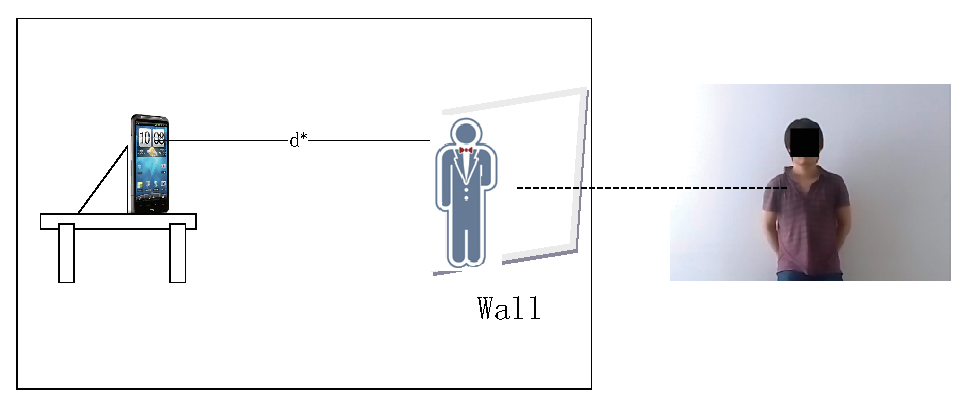
\includegraphics[width=3.5in]{epsfacedistance.eps}
\caption{Experimental setup for evaluation of distance estimation based on face detection}
\label{fig:distance-exp}
\end{figure}


Fig.~\ref{fig:distance-results} shows that the estimated distance is close to the actual distance using different phones.  The accuracy of distance estimation achieves nearly 82\%.
The error is caused by deviation in mapping image pixel count to actual distance.  We also observe that different phones have similar degree of accuracy.
By assuming the real face height  as 22cm (i.e., 8.734 inches), we use Eq.(2) to calculate the distance between camera and the face, which is 2.938m, very close to the actual distance of 2.4m.  We also calculate the area size to be 3.407$m^2$ while the actual size is 2.318$m^2$. This area estimation error is acceptable for detecting visual eavesdroppers.
%Fig.~\ref{fig:area-results} shows that the estimated area size is close to the actual area size using different phones.


\begin{figure}[H]\label{exp:expdistancechart}
\centering
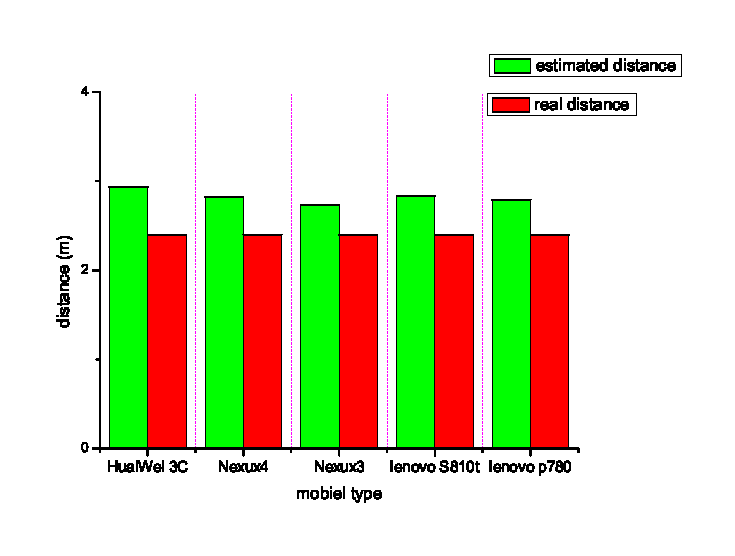
\includegraphics[width=2.7in]{epsdistancechart1.eps}
\caption{Estimated and actual distance of different phones}
\label{fig:distance-results}
\end{figure}

\begin{comment}
\begin{figure}[H]
\centering
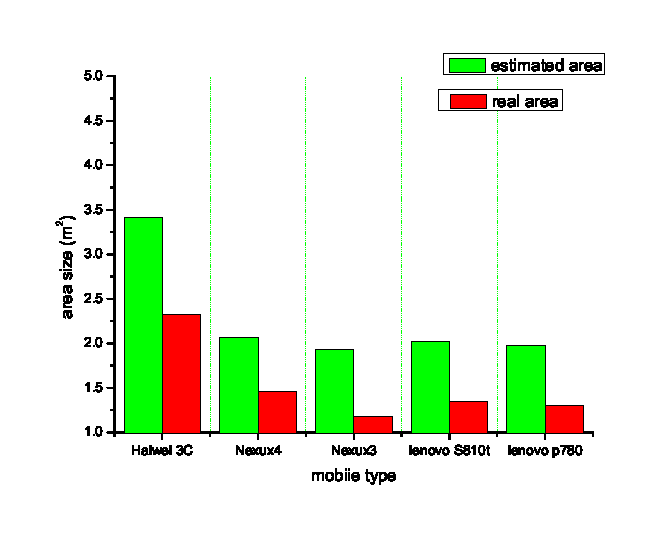
\includegraphics[width=2in]{epsdistancechart2.eps}
\caption{Estimated and actual monitoring area size of different phones}
\label{fig:area-results}
\end{figure}
\end{comment}

\subsection{Experiments on Face and Motion Detection} % Inside Camera View}
We use  publicly available face datasets such as BioID\cite{BioID}, Caltech\cite{jesorsky2001robust}, and FDDB\cite{jain2010fddb} datasets to evaluate the performance of our face detection, use the motion detection or tracking dataset such as PETS\cite{website:PETS} and part of the Yhyang tracking datasets to evaluate the performance of motion detection.

Our face detection achieves an accuracy of $81.7\%$, $95.3\%$ and $98.5\%$  using the FDDB, Caltech, and  BioID datasets respectively. Fig.~\ref{fig:face-results} is a sample of the face detection results. We observe the decrease of face detection accuracy with the lower clarity of the face in the image either due to presence of multiple faces in the images or low resolution of the image. We also notice that the face detection method always fails while the face does not directly face the camera.
\begin{figure}[H]
\centering
\includegraphics[width=3in]{epsfaces.eps}
\caption{Face detection results using publicly available datasets}
\label{fig:face-results}
\end{figure}

 The motion detection method achieves a high accuracy of more than $90\%$ using the classical datasets PETS2001. Fig.~\ref{fig:motion-results} is a sample result of motion detection. However, the method detects any moving object, not limited to moving person.  Since we are only interested in human, we combine  face detection  and motion detection.
 \begin{figure}[H]
\centering
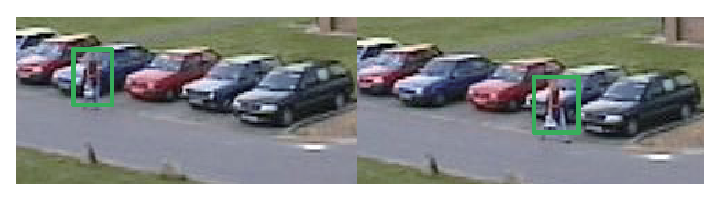
\includegraphics[width=3.5in]{epsmotionret.eps}
\caption{The experiments on motion detection in the PETS2001 datasets. }
\label{fig:motion-results}
\end{figure}


To evaluate the efficiency of our face detection which first removes the user-blocked area, we compare it against the method without blocked area removal  using images in the Caltech face datasets. The resolution of each image is $800\times600$, which is high enough to test the speed of face detection.  Fig.~\ref{fig:blocked-results} shows that our face detection method saves almost 20\% of the computation.
 \begin{figure}[H]
\centering
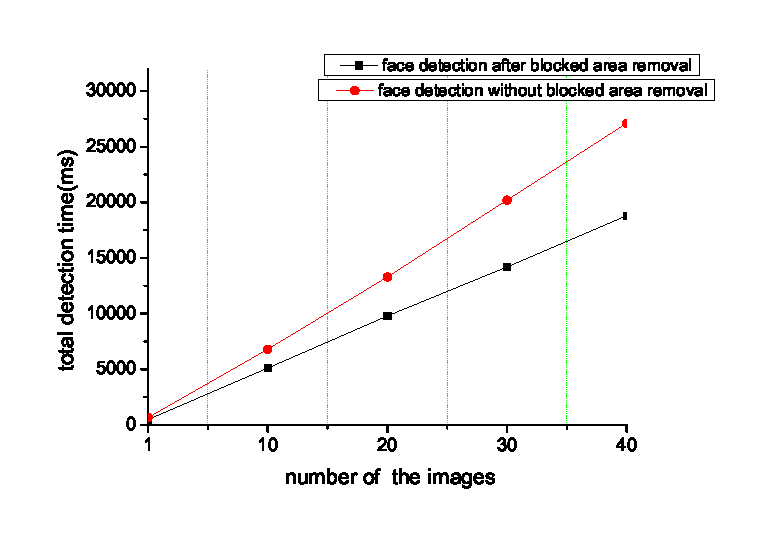
\includegraphics[width=3in]{epsfaceremoval.eps}
\caption{Face detection time}
\label{fig:blocked-results}
\end{figure}


\subsection{Experiments on Prediction of Visual Eavesdropper Location }


For predicting the location of a visual eavesdropper,  motion speed and direction is important to estimate the probability of the existing visual eavesdropping. In most situations,  motion direction takes a simple form, i.e., moving either left or right. Compared with  motion direction,  motion speed is more important in predicting the location of the visual eavesdropping. Therefore, we conduct the experiments on estimating motion speed to evaluate the accuracy of our method.

As Fig.~\ref{fig:speed-exp} shows, we let a person stand by the wall and go from  left  to  right. We record the time from the motion start to the motion end for several times. The width of the wall is 6.5 m and the speed can be calculated by dividing the length by the time. The average time is 7.5 seconds and the speed is 0.86 m/s. For our motion speed estimation, we use face detection method to locate the initial human position and consider the area that is three times of the face size,  below the face is the human body. We then use motion detection to track the human that includes the human face and body for getting the trajectories.

\begin{figure}[H]
\centering
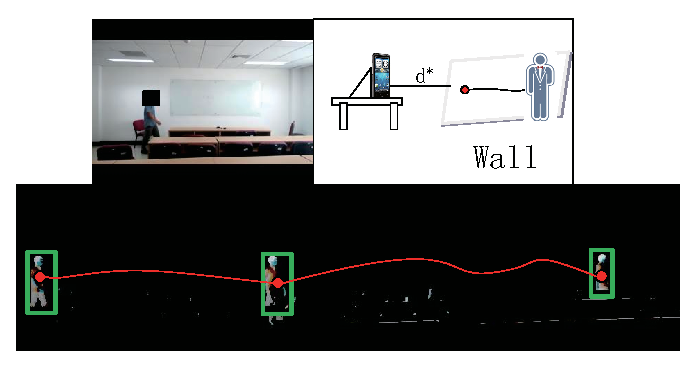
\includegraphics[width=3.5in]{epsmotion.eps}
\caption{Experimentsal setup for evaluating motion speed estimation. }
\label{fig:speed-exp}
\end{figure}
Considering that the distance $d^*$ is important for estimating the motion speed, we estimate the motion speed with known distance $d^*$ and also estimate motion speed in a designated area using time.
Fig.~\ref{fig:speed-results1} shows the estimated motion speed is close to the actual speed and achieves nearly $91.3\%$.




\begin{comment}
\subfigure{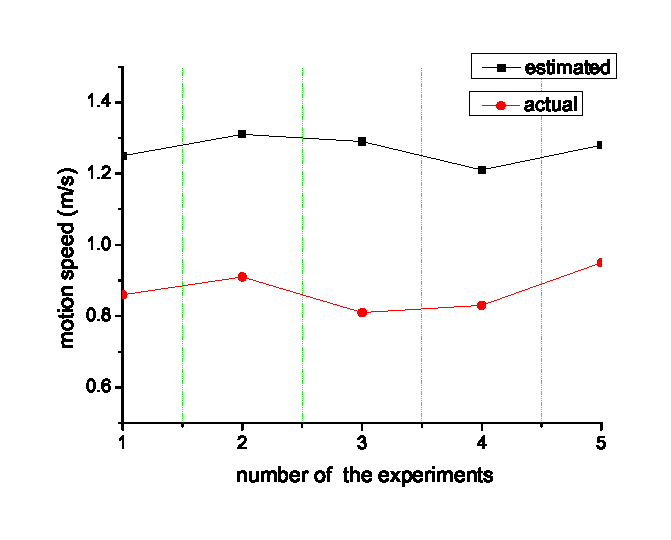
\includegraphics[width=3in]{epsmotionchart2.eps}}
\caption{Estimation of motion speed with estimated distance}
\label{fig:speed-results2}
\end{comment}


\subsection{Experiments on Overall Visual Eavesdropper Detection}
All the experiments discussed previously demonstrate that each component of our proposed visual eavesdropper detection method (i.e., area estimation, visible human detection,  and location prediction)  performs well using public datasets.  To validate that our overall approach works well in practice, we conducted the following experiments. We ask one person to use his phone as usual and another person tries to read his phone screen from behind while walking slowly behind him from left to right.
we set the angle of the camera view $\alpha_h$, $\alpha_v$ to $ 30^\circ $, $ 22^\circ $ and set the angle of potential eavesdropping $\beta$ to $ 60^\circ $. In this experiment, the time threshold \textit{t}(s) and $\tau(s)$  %learned by sensitivity of the environment perception
are set to be $12s$ and $8s$ respectively.  Fig.~\ref{fig:all-results} shows the results of these experiments.
The black area is the area blocked by phone user's face. The left figure shows  that the person behind the user is detected by face detection where the small rectangle is the detected human face; the right figure shows that the person is tracked by motion detection although the face is not detected where the large rectangle is the tracked human body. When the person moves out of the monitoring area, we get the probability to visual eavesdropping. When the time of the detected face is more than  threshold $\tau(s)$ or the time of the detected body is more than  threshold \textit{t}(s), the person behind is considered as a visual eavesdropper. The result of this experiment validates the effectiveness of our proposed visual eavesdropper detection.
\begin{figure}[H]
\centering
\includegraphics[width=3.5in]{expvee.eps}
\caption{Experiments on visual eavesdropper detection }
\label{fig:all-results}
\end{figure}


%{\bf Performance Summary. } Our finding include: (1) The area size calculated by the area estimation method is close to the real area size. (2) The estimation of the motion detection result can get approximate the motion speed and direction.(3) Proposed Human detection method has a robust detection result in the datasets.
